\documentclass[12pt]{article}

\usepackage{amssymb,amsmath,amsthm}
\usepackage{graphicx} % Package for including figures
%\usepackage{psfrag,color}
\graphicspath{ {.}}

\theoremstyle{definition}
\newtheorem{thm}{Theorem}[section]
\newtheorem{lem}[thm]{Lema}
\newtheorem{prop}[thm]{Proposition}
\newtheorem*{cor}{Corrolary}

\theoremstyle{definition}
\newtheorem{defn}{Definition}[section]
\newtheorem{conj}{Conjecture}[section]
\newtheorem{exmp}{Example}[section]


\title{Report: Homework 6 Math/CS 471}
\author{Teo Brandt and Brennan Collins}
\date{\today}   % Activate to display a given date or no date


\begin{document}
\maketitle

\begin{abstract}
This report will discuss the importance of parallel programming as well as provide an example of the implementation of parallelism on a previous program that was introduced in the report on Homework 4. The goal of this report is to quantify parallelism.
\end{abstract}

\section{How to Quantify Parallelism}
The first measure that will be introduced is referred to as \textbf{speedup}. Suppose we run a code on a single processor and it takes \(T_{1}\) time to run, then if we run it on \(p\)-processors we can define the speedup as
\[
S_{p}=\frac{T_{1}}{T_{p}}
\]
The ideal speedup occurs when \(S_{p}={p}\). Another measure that is important to introduce is the \textbf{efficiency} defined as
\[
\text{Efficiency: }\frac{S_{p}}{p}
\]
Another area that will be discussed later in this report is that of \textbf{strong} and \textbf{weak scaling}. When the problem size is fixed the computation of the speedup and efficiency for various sized problems is known as weak scaling. On the other hand, when the problem size specifically allocated to a particular processor is called strong scaling. To observe strong scaling one must fix the work per processor and increase the number of processors then choose the size of the problem accordingly. The last measure of computation is simply the number of floating points per second that are being computed. This measure can be obtained by counting the number of floating point operations in a particular routine and dividing this number by the total computational time. The idea is the better results (or rather the better program) is one that involves close proximity to the theoretical maximum speedup.

\section{Program: Homework 4's Mapping}
As discussed in the report for homework 4 when approximating derivatives over an abstract region one choice is to compute the spatial derivatives using finite differences \(\frac{\delta u}{\delta x} (x) \approx \frac{u(x+h)-u(x)}{h}\). As well as computing the derivatives over a region the program that is to be parallelized here computes integrals on the reference element and then compares the numerically obtained result with the known, or exact solution.

\section{Parallelizing}
In order to parallelize the code from Homework 4 OpenMP was used. OpenMP is a collection of compiler directives and library routines for parallel shared memory \cite{HW}. The reason that OpenMP is used is because the implementation of directive sentinels allows a program that is initially a serial code and to covert it in such a way that it may still be ran in serial mode. These sentinels are \(!\$OMP\) and \(!\$\). When a non-OpenMP compiler runs into these characters it sees the lines as comments. Herein lies the usefulness because the sentinels lead to conditional compiling that may either have one behavior or another depending on the compiler chosen.

\section{Results}
The first thing that was done was the verification that the code described in the previous section, after being parallelized, can still be ran in serial and provides the same result independent of the number of processors being utilized. Shown in the figure below is the initial run of the code with output consisting of computational time, error, and the number of strings being used.
\begin{figure}[h]
\caption{Screen image}
\centering
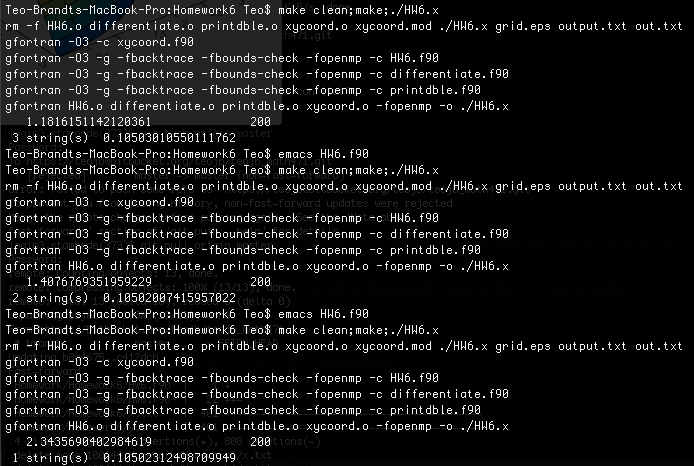
\includegraphics[width=0.75\textwidth]{initialresults}
\end{figure}
\newpage
These initial results display the expected behavior as time decreases with an increase in the number of processors. Additionally the speedup seen here was roughly \(S_{3}=1.983360751\) and \(S_{2}=1.664848647\) with respective efficiencies \(e_{3}=0.6611\) and \(e_{2}=0.8324\). The capabilities of the computer used to obtain these initial results are limited to 4 cores and in the next section the supercomputer Xsede will be introduced and the results obtained from its use will be presented.

\section{Xsede}
The results from Xsede are included in the directory with the code as described in the appendix.

\section{Appendix}
To run the program, simply navigate to Homework6/Code and enter the command "make" followed by "./HW6.x". The results are printed to the screen as shown by Figure 1 above.
\\

\newpage
\begin{thebibliography}{9}
\bibitem{HW} 
Daniel Appelo
\textit{Homework 3}. 
referenced Oct. 29, 2015

\end{thebibliography}

\end{document} 